
\section{Integration with the Lightning Network}\label{lninte}

While having the protocol presented in Section~\ref{offdlcproto} theoretically enables the creation of DLC channels, implementing all the necessary infrastructure would require a lot of additional work.
A lot of this work has already been carried on by the many researchers and developers who have contributed to the development of the Lightning Network.
Leveraging this work, and new or on-going research such as channel splicing, sub-marine swaps or channel factories~\cite{burchert2018scalable} for the creation of DLC channels would thus reduce the required effort.

In addition, if two parties who already have an established Lightning Network channel open with each others wished to create a DLC channel, it would be impractical and wasteful for them to have to broadcast another fund transaction.
Another issue arises if the parties wish to establish several contracts concurrently, as this would require opening several channels between the two parties.
Finally, as two parties participate in consecutive contracts within a DLC channel, it might become imbalanced, preventing further contracts to take place.

In this section, we propose a way to integrate DLC channels within the Lightning Network to enable:
* Reusing the Lightning Network infrastructure for peer discovery, channel funding, as well as recent innovations such as channel factories or splicing,
* the two parties of a lightning channel to establish multiple DLC channels in parallel to the lightning one, reusing the same fund transaction,
* the reallocation of funds between a lightning channel and DLC channels.

An illustration of the transactions for the integration of a single DLC channel with a lightning one is given in Figure~\ref{fig:lnin}.

\begin{figure*}
  \centering
  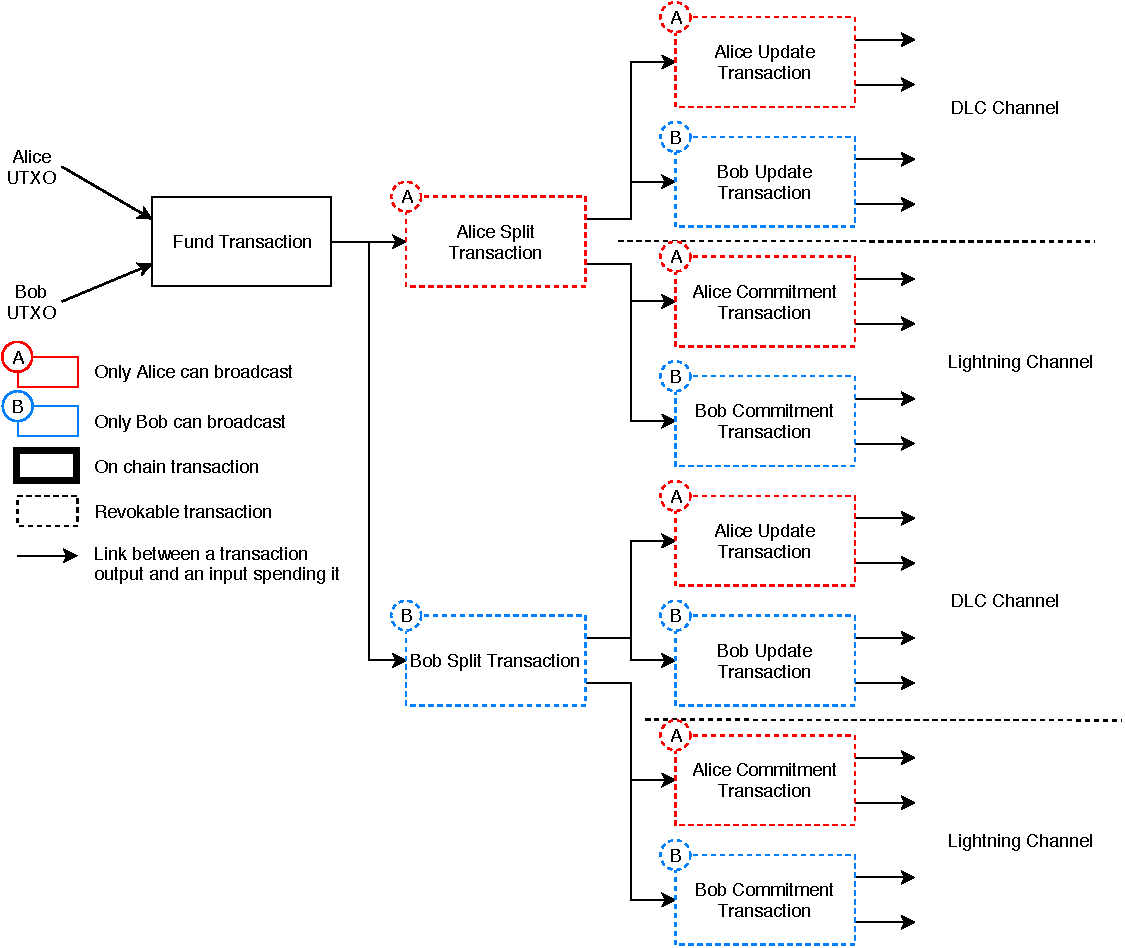
\includegraphics[width=\textwidth]{Figures/LightningIntegration.pdf}
  \caption{Illustration of the transaction construction for splitting a channel into a DLC and lightning one.}
  \label{fig:lnin}
\end{figure*}

\subsection{Split transaction}

To divide the allocation of funds from the fund transaction to both the lightning and DLC channels, we introduce a \emph{split transaction}.
This transaction contains multiple outputs, one for the funding of the lightning channel, and one for the funding of each of the DLC channels, each with a revocation path and a multi signature path (detailed in Script~\ref{script:splittx}).
Due to the revocation paths, each party needs to hold a different version of a split transaction.

\subsection{Channel splitting}

Here we assume that a dual funded lightning channel already exists between Alice and Bob, that they wish to establish a single DLC channel in parallel (the protocol generalizes to multiple ones), and that they have agreed on how much funds to allocate to each channel.
The protocol for a channel split is as follow:
\begin{enumerate}
  \item Alice sends signatures for Bob's update (for the DLC channel), commitment (for the lightning channel) and split transactions,
  \item Bob sends signatures for Alice's update, commitment and split transactions, as well as the secret for his previous commitment transaction,
  \item Alice sends the secret to her previous commitment transaction,
  \item Alice and Bob follow a protocol similar to presented in Section~\ref{offdlcproto} to finish the establishment of the DLC channel, with the difference of having to handle four sets of transactions instead of two (due to the asymmetry of the \emph{split transaction}).
\end{enumerate}

Subsequently, both channels can be updated independently.

If Alice and Bob wish to re-balance the funds between the lightning and DLC channels, they can follow a similar protocol, but revoke the split transactions instead of the initial commitment transactions of the lightning channel.

Finally, they can also close the DLC channel and return to a simple lightning channel by creating new commitment transactions allocating the sums of the funds of each party in each channel before revoking the \emph{split transaction}.

\subsection{Discussion}\label{discuss}

One of the main drawback of our proposed split channel design, is the larger amount of transactions to keep track of.
This increases the complexity of the system as well as the burden for watchtowers~\cite{khabbazian2019}.

Another approach to integrate DLC channels together with lightning channel would be to use an extra output in the lightning channel's commitment transaction, that can be used as a funding input to a DLC.
This was proposed by Bedn\'ar and Pickhardt~\cite{bednar2019}.
While it does effectively reduce the number of transactions, it also means that for each update of the lightning channel, all the transactions for the DLC need to be reconstructed, signed and exchanged.
The update of each channel also becomes dependent on the state of the other channel, potentially leading to concurrency issues.
We thus believe that the extra cost induced by the split of the channel is compensated by a better separation between the two channels and the ability to update them independently.

We also note that this splitting approach, while designed in the context of allowing DLC channels within the Lightning network, could also be used to integrate other types of channel relying on a fund transaction.